% A LaTeX template for EXECUTIVE SUMMARY of the MSc Thesis submissions to
% Politecnico di Milano (PoliMi) - School of Industrial and Information Engineering
%
% P. F. Antonietti, S. Bonetti, A. Gruttadauria, G. Mescolini, A. Zingaro
% e-mail: template-tesi-ingind@polimi.it
%
% Last Revision: October 2021
%
% Copyright 2021 Politecnico di Milano, Italy. Inc. All rights reserved.

\documentclass[11pt,a4paper]{article}

%------------------------------------------------------------------------------
%	REQUIRED PACKAGES AND  CONFIGURATIONS
%------------------------------------------------------------------------------
% PACKAGES FOR TITLES
\usepackage{titlesec}
\usepackage{color}

% PACKAGES FOR LANGUAGE AND FONT
\usepackage[utf8]{inputenc}
\usepackage[english]{babel}
\usepackage[T1]{fontenc} % Font encoding

% PACKAGES FOR IMAGES
\usepackage{graphicx}
\graphicspath{{Images/}} % Path for images' folder
\usepackage{eso-pic} % For the background picture on the title page
\usepackage{subfig} % Numbered and caption subfigures using \subfloat
\usepackage{caption} % Coloured captions
\usepackage{transparent}

% STANDARD MATH PACKAGES
\usepackage{amsmath}
\usepackage{amsthm}
\usepackage{bm}
\usepackage[overload]{empheq}  % For braced-style systems of equations

% PACKAGES FOR TABLES
\usepackage{tabularx}
\usepackage{longtable} % tables that can span several pages
\usepackage{colortbl}

% PACKAGES FOR ALGORITHMS (PSEUDO-CODE)
\usepackage{algorithm}
\usepackage{algorithmic}

% PACKAGES FOR REFERENCES & BIBLIOGRAPHY
\usepackage[colorlinks=true,linkcolor=black,anchorcolor=black,citecolor=black,filecolor=black,menucolor=black,runcolor=black,urlcolor=black]{hyperref} % Adds clickable links at references
\usepackage{cleveref}
\usepackage[square, numbers, sort&compress]{natbib} % Square brackets, citing references with numbers, citations sorted by appearance in the text and compressed
\bibliographystyle{plain} % You may use a different style adapted to your field

% PACKAGES FOR THE APPENDIX
\usepackage{appendix}

% PACKAGES FOR ITEMIZE & ENUMERATES
\usepackage{enumitem}

% OTHER PACKAGES
\usepackage{amsthm,thmtools,xcolor} % Coloured "Theorem"
\usepackage{comment} % Comment part of code
\usepackage{fancyhdr} % Fancy headers and footers
\usepackage{lipsum} % Insert dummy text
\usepackage{tcolorbox} % Create coloured boxes (e.g. the one for the key-words)
\usepackage{stfloats} % Correct position of the tables
\usepackage{multirow}
\usepackage{multicol}
\usepackage{twemojis}
\usepackage{fontawesome}
\usepackage{listings}
\usepackage{guit}

\usepackage{tikz}
\usetikzlibrary{positioning, arrows.meta}



%-------------------------------------------------------------------------
%	NEW COMMANDS DEFINED
%-------------------------------------------------------------------------
% EXAMPLES OF NEW COMMANDS -> here you see how to define new commands
\newcommand{\bea}{\begin{eqnarray}} % Shortcut for equation arrays
\newcommand{\eea}{\end{eqnarray}}
\newcommand{\e}[1]{\times 10^{#1}}  % Powers of 10 notation
\newcommand{\mathbbm}[1]{\text{\usefont{U}{bbm}{m}{n}#1}} % From mathbbm.sty
\newcommand{\pdev}[2]{\frac{\partial#1}{\partial#2}}
\newlength{\dunder}
\setlength{\dunder}{0.5em}
\newcommand{\twound}{\rule{2\dunder}{0.4pt}}
% NB: you can also override some existing commands with the keyword \renewcommand

%----------------------------------------------------------------------------
%	ADD YOUR PACKAGES (be careful of package interaction)
%----------------------------------------------------------------------------
\usepackage{amsfonts} 

%----------------------------------------------------------------------------
%	ADD YOUR DEFINITIONS AND COMMANDS (be careful of existing commands)
%----------------------------------------------------------------------------


% Do not change Configuration_files/config.tex file unless you really know what you are doing.
% This file ends the configuration procedures (e.g. customizing commands, definition of new commands)
% Set the geometric layout of the document
\usepackage{geometry}
\geometry{
  top=3cm,
  left = 2.0cm,
  right = 2.0cm,
  bottom=2cm,
  headheight= 2cm,
  headsep= 0cm,
}
\raggedbottom

% Create color bluePoli (-> manuale grafica coordinata:  https://www.polimi.it/fileadmin/user_upload/il_Politecnico/grafica-coordinata/2015_05_11_46xy_manuale_grafica_coordinata.pdf)
\definecolor{bluePoli}{cmyk}{0.4,0.1,0,0.4}

% Custom theorem environments
\declaretheoremstyle[
  headfont=\color{bluePoli}\normalfont\bfseries,
  bodyfont=\color{black}\normalfont\itshape,
]{colored}

\captionsetup[figure]{labelfont={color=bluePoli}} % Set colour of the captions
\captionsetup[table]{labelfont={color=bluePoli}} % Set colour of the captions
\captionsetup[algorithm]{labelfont={color=bluePoli}} % Set colour of the captions

\theoremstyle{colored}
\newtheorem{theorem}{Theorem}[section]
\newtheorem{proposition}{Proposition}[section]

% Enhances the features of the standard "table" and "tabular" environments.
\newcommand\T{\rule{0pt}{2.6ex}}
\newcommand\B{\rule[-1.2ex]{0pt}{0pt}}

% Algorithm description
\newcounter{algsubstate}
\renewcommand{\thealgsubstate}{\alph{algsubstate}}
\newenvironment{algsubstates}{
    \setcounter{algsubstate}{0}%
    \renewcommand{\STATE}{%
    \stepcounter{algsubstate}%
    \Statex {\small\thealgsubstate:}\space}
    }{}

% Custom theorem environment
\newcolumntype{L}[1]{>{\raggedright\let\newline\\\arraybackslash\hspace{0pt}}m{#1}}
\newcolumntype{C}[1]{>{\centering\let\newline\\\arraybackslash\hspace{0pt}}m{#1}}
\newcolumntype{R}[1]{>{\raggedleft\let\newline\\\arraybackslash\hspace{0pt}}m{#1}}

% Custom itemize environment
\setlist[itemize,1]{label=$\bullet$}
\setlist[itemize,2]{label=$\circ$}
\setlist[itemize,3]{label=$-$}
\setlist{nosep}

% Set separation of columns
\setlength{\columnsep}{30pt}

% Create command for background pic
\newcommand\BackgroundPic{% Adding background picture
	\put(230,358){
		\parbox[b][\paperheight]{\paperwidth}{%
			\vfill
			\centering
			\transparent{0.4}
			
\includegraphics[width=0.5\paperwidth]{raggiera_polimi.eps}%
			\vfill
}}}

% Set indentation
%\setlength\parindent{0pt}

% Custom title commands
\titleformat{\section}
{\color{bluePoli}\normalfont\Large\bfseries}
{\color{bluePoli}\thesection.}{1em}{}
\titlespacing*{\section}
{0pt}{2ex}{1ex}

\titleformat{\subsection}
{\color{bluePoli}\normalfont\large\bfseries}
{\color{bluePoli}\thesubsection.}{1em}{}
\titlespacing*{\subsection}
{0pt}{2ex}{1ex}

\titleformat{\subsubsection}
{\color{bluePoli}\normalfont\normalsize\bfseries}
{\color{bluePoli}\thesubsubsection.}{1em}{}
\titlespacing*{\subsubsection}
{0pt}{2ex}{1ex}

% Custom headers and footers
\pagestyle{fancy}
\fancyhf{}

\fancyfoot{}
\fancyfoot[C]{\thepage} % page
\renewcommand{\headrulewidth}{0mm} % headrule width
\renewcommand{\footrulewidth}{0mm} % footrule width

\makeatletter
\patchcmd{\headrule}{\hrule}{\color{black}\hrule}{}{} % headrule
\patchcmd{\footrule}{\hrule}{\color{black}\hrule}{}{} % footrule
\makeatother

% -> Create the header
\chead[C]{
\centering
\begin{tcolorbox}[arc=0pt, boxrule=0pt, colback=bluePoli!60, width=\textwidth, colupper=white]
    % \textbf{Homework 1} \hfill \textbf{\author}  
\end{tcolorbox}
}


% Insert here the info that will be displayed into your Title page
% -> title of your work
\renewcommand{\title}{Title}

% -> author name and surname
\renewcommand{\author}{Andrea Bonifacio, Sara Gazzoni}
% -> MSc course
\newcommand\norm[1]{\lVert#1\rVert}
\newcommand{\course}{Advanced Programming for Scientific Computing}
% -> advisor name and surname
\newcommand{\advisor}{Stefano Pagani}
% IF AND ONLY IF you need to modify the co-supervisors you also have to modify the file Configuration_files/title_page.tex (ONLY where it is marked)
\newcommand{\firstcoadvisor}{Mattia Corti} % insert if any otherwise comment
%\newcommand{\secondcoadvisor}{Name Surname} % insert if any otherwise comment
% -> academic year
\newcommand{\YEAR}{2022-2023}

%-------------------------------------------------------------------------
%	BEGIN OF YOUR DOCUMENT
%-------------------------------------------------------------------------
\begin{document}

%-----------------------------------------------------------------------------
% TITLE PAGE
%-----------------------------------------------------------------------------
% Do not change Configuration_files/TitlePage.tex (Modify it IF AND ONLY IF you need to add or delete the Co-advisors)
% This file creates the Title Page of the document
% DO NOT REMOVE SPACES BETWEEN LINES!

%\twocolumn[{\begin{@twocolumnfalse}

\AddToShipoutPicture*{\BackgroundPic}

\hspace{-0.6cm}
\includegraphics[width=0.6\textwidth]{logo_polimi_ing_indinf.eps}

\vspace{-1mm}
\fontsize{0.3cm}{0.5cm}\selectfont \bfseries \textsc{\color{bluePoli} Project Report}\\

\vspace{-0.2cm}
\Large{\textbf{\color{bluePoli}{\title}}}\\

\vspace{-0.2cm}
\fontsize{0.3cm}{0.5cm}\selectfont \bfseries \textsc{\color{bluePoli} \course}\\

\vspace{-0.2cm}
\fontsize{0.3cm}{0.5cm} \selectfont \bfseries Authors: \textsc{\textbf{\author}}\\

\vspace{-0.4cm}
\fontsize{0.3cm}{0.5cm}\selectfont \bfseries Advisors: \textsc{\textbf{\advisor}}\\

% if only ONE co-advisor is present:
\vspace{-0.4cm}
\fontsize{0.3cm}{0.5cm}\selectfont \bfseries Co-advisor: \textsc{\textbf{\firstcoadvisor}}\\
% if more than one co-advisors are present:
%\vspace{-0.4cm}
%\fontsize{0.3cm}{0.5cm}\selectfont \bfseries Co-advisors: \textsc{\textbf{\firstcoadvisor}}\textsc{\textbf{\secondcoadvisor}}\\

\vspace{-0.4cm}
\fontsize{0.3cm}{0.5cm}\selectfont \bfseries Academic year: \textsc{\textbf{\YEAR}}

\small \normalfont

\vspace{11pt}

\centerline{\rule{1.0\textwidth}{0.4pt}}

%\vspace{15pt}
%\end{@twocolumnfalse}}]

\thispagestyle{plain} % In order to not show the header in the first page


%%%%%%%%%%%%%%%%%%%%%%%%%%%%%%
%%     THESIS MAIN TEXT     %%
%%%%%%%%%%%%%%%%%%%%%%%%%%%%%%

%-----------------------------------------------------------------------------
% INTRODUCTION
%-----------------------------------------------------------------------------

\section{Introduction}
Full 3D blood flow models are important in the study of the cardiovascular system since they allow one to extract detailed quantities of interest, but their actual implementation is limited due to their high computational cost. For this reason, reduced order models are widely used in this field because of their efficiency. An example is presented in \cite{Luca}, where a one-dimensional reduced order model is implemented to simulate the blood flow in the aorta using a graph neural network trained on three-dimensional simulations. In this work we propose a different application, where the graph neural network is used to approximate the solution of different problems. In particular, we consider the heat equation as test case, but the goal of the project is to show the potential extension of this approach to solve more difficult problems with complex geometries such as the simulations of proteins spreading in the neural system, which are at the basis of neurodegenerative diseases \cite{MattiaCorti}. The main part of this project is the implementation of a library for data generation used to train the graph neural network, and the adaptation of the code\footnote{The code can be found \href{https://github.com/StanfordCBCL/gROM}{here}.} used in the paper\cite{Luca} to make it suitable for our specific test case. In the following sections, we first present the problem formulation and a detailed description of the code developed, then we show the results obtained and a discussion of the possible further developments and extensions.

%-----------------------------------------------------------------------------
% Problem
%-----------------------------------------------------------------------------

\section{Problem overview}

% descrizione del problema generico Lu=F risolto con Fenics
We consider a general time-dependent variational problem of the form:
\[Lu=f\]
with \(L\) a linear operator, \(f\) a source term and \(u\) the solution. Given a specific geometry \(\Omega\) and using the finite element method implemented in FEniCS, we can solve this problem and obtain the solution \(u^{n}\) at each time step \(n\). From this, we can generate a graph that describes the geometry of the problem and the solution, storing some values of interest as features of the nodes and the edges. By solving the problem for different geometries and different values of the parameters (e.g. the diffusivity constant) we can generate a dataset that will be used to train the graph neural network. 

The graph neural network used in this project is the one presented in \cite{Luca}, which is an adaptation of the MeshGraphNet implementation \cite{MeshGraphNet}, and that we modified to make it suitable for our test case and extendable to other problems.

The GNN is applied iteratively: at each time step it takes as input the system state \(\Theta^{n}\), which is the set of all the nodes and edges features at that time step, and it predicts an update for the state variables (rollout phase). The prediction is combined with the previous time step to estimate \(\Theta^{n+1}\). 
A forward step of the GNN is composed by three stages:
\begin{enumerate}
    \item Encode: a latent representation of the node and edge features is computed using a fully connected neural network.
    \item Process: the process stage is composed by L identical blocks, each of them is applied in sequence to the output of the previous blocks, updating the node and edge features. 
    \item Decode: using a fully connected neural network, the node features are transformed from the latent space to the output space. The output of the GNN is a vector containing the update of the state variables \(\delta\Theta^n\) at each node of the graph. 
\end{enumerate}
After this forward step, the state variables can be updated as \(\Theta^{n+1} = \Theta^{n} + \delta\Theta^{n}\).

We consider our dataset composed of \(G\) graphs, each of them consisting of a set of nodes \(n_1^g,...,n_{N^g}^g\), and we define as \(M^g\) the final time step of the \(g\)-th graph.
The neural network is trained on small strides \(s\) of consecutive timesteps since it has been proven to improve the accuracy of the predictions \cite{Luca}.
The loss function minimized during the training is defines as:
\begin{equation}
    \mathcal{L} = \sum_{g \in \mathcal{T}} \frac{1}{|\mathcal{T}|(M^g-s)} \sum_{n=0}^{M^g-s} sMSE^{n,g,s},
\end{equation}
where \(\mathcal{T}\) is the set of graphs used for training and \(sMSE\) is the strided mean squared error between the prediction and the ground truth:
\begin{equation}
    sMSE^{n,g,s} = \frac{1}{N^g} \sum_{l=1}^{s} \sum_{i=1}^{N^g} a_l (\hat{\Theta}^{k+l,g} - \Phi_l(\Theta^{k,g}|_i))^2.
    \label{mse}
\end{equation}
In the above equation, \(a_l=1\) if \(l=1\) and \(a_l=0.5\) otherwise, \(\hat{\Theta}^{k+l,g}\) is the exact value of the nodal state variable at time step \(k+l\) of the \(g\)-th graph, and \(\Phi_l(\Theta^{k,g}|_i)\) is the approximation of \(\Theta\) at node \(i\) after \(l\) application of the GNN. 
The loss function is optimized using the Adam optimizer.

During the training, the state variables are perturbed with random noise to simulate the error caused by the network's predictions, this is done to improve the robustness of the network and we have hyperparameters to control the rate of the noise. 

It is important to make the graph neural network robust for rollouts of many time steps, since the error generated by the predictions is propagated at each time step. 
For this reason, in addition to the loss function, to evaluate the performance of the network we compute also the rollout error, which is defined as: 

\begin{equation}
    e^g = \frac{ \sum_{i=1}^{N^g} \sum_{k=11}^{M^g} (\hat{\Theta}_i^{k,g} -  \Phi_l(\Theta^{k,g}|_i))^2 }{ \sum_{i=1}^{N_g} \sum_{k=1}^{M^g} (\hat{\Theta}_i^{k,g})^2 }.
    \label{rollout}
\end{equation}


\subsection{Test case: heat equation}
\label{testcase}

In this work, we consider the heat equation as test case. 
The mathematical formulation of the problem is the following:
\begin{equation}
    \begin{cases}
        \frac{\partial u }{\partial t} = k \Delta u \quad \text{in} \ \Omega \subset \mathbb{R}^2, \\
        \frac{\partial u}{\partial n} = h \quad \text{on} \ \partial \Omega_{inlet}, \\
        \frac{\partial u}{\partial n} = 0 \quad \text{on} \ \partial \Omega_{outlet} 
        \cup \partial \Omega_{walls}.
    \end{cases}
\end{equation}
where \(u\) is the temperature, \(k\) is the diffusivity constant, \(h\) is the Neumann condition at the inlet boundary. As domain \(\Omega\) we consider different geometries such as the one shown in Figure \ref{mesh}: the 2D mesh is composed of 4 trapezoids where the interface between them have different lengths. The inlet boundary is the left one, while the outlet boundary is the right one. The other two boundaries are the walls.

\begin{figure}[H]
    \centering
    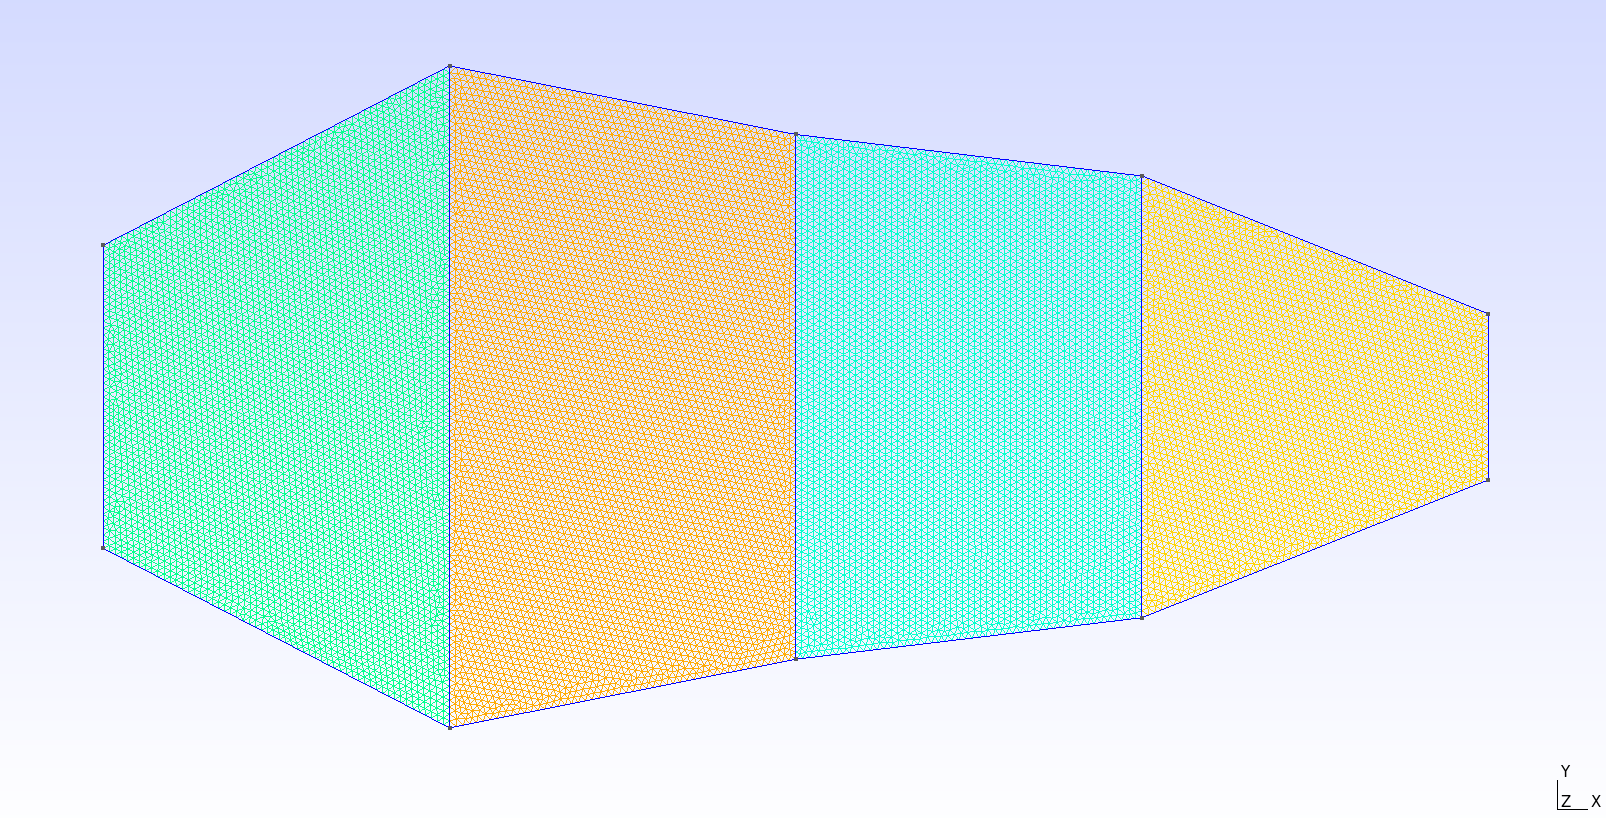
\includegraphics[width=0.4\textwidth]{Images/mesh.png}
    \caption{Example of a mesh used in the test case.}
    \label{mesh}
\end{figure}

We generated 20 different mesh using gmsh. 
Then we solved the problem in FEniCS using Discontinuous Galerkin method and implicit Euler for time discretization, imposing as Neumann condition at inlet \(h = 2e^{-(t-2.5)^2}\).
From these solutions we generated a dataset of 277 graphs. 
Each graph has 5 nodes: an inlet node, an outlet node and 3 nodes in correspondence of the interfaces. 
As descriptor of the state of the system we consider the heat flux at each time step, which is computed as the integral of the normal derivative of the temperature on the interface. The other node features are the thermal diffusivity \(k\), the interface length and the nodal type (inlet, outlet or branch node). 
As edge features we consider the area of the corresponding trapezoid and the distance between the nodes connected by the edge. 
The graph neural newtork is trained for 300 epochs on this dataset, a list of the hyperparameters used is shown in Table \ref{hyperparams}. To more details about the hyperparameters and the network architecture we refer to Section \ref{gnn}.

\begin{table}[H]
    \centering
    \begin{tabular}{|c|c|}
        \hline
        \textbf{Parameter} & \textbf{Value} \\
        \hline
        batch size & 32 \\
        learning rate decay & 0.001 \\
        learning rate & 0.01 \\
        rate noise & 5 \\
        rate noise features & \(10^{-5}\) \\
        l2 regularization & \(10^{-5}\) \\
        latent size gnn & 8 \\
        latent size mlps & 16\\
        normalization type & 1 (normal) \\
        stride & 5 \\
        \hline   
    \end{tabular}
    \caption{Hyperparameters used for the GNN training.}
    \label{hyperparams}
\end{table}

%-----------------------------------------------------------------------------
% Code
%-----------------------------------------------------------------------------

\section{Code}

The implementation of this work is in Python. The mesh generation is done using \texttt{gmsh}, while the variational problem is solved using \texttt{FEniCS}. The graph neural network is implemented using \texttt{PyTorch}. The code is available on GitHub\footnote{The repository can be found}. %\href{mettere il link}}.

\noindent
The folders and files in the repository are organized as follows:
\medskip
\begin{itemize}
    \item[\faFolder] \textbf{scripts}: this folder contains the scripts with all the classes and functions necessary to create the meshes, solve the variational problems and generate the graphs. 
    \medskip
    \item[\faFolder] \textbf{gNN}: this folder contains the code of the graph neural network.
    \medskip
    \item[\faFolder] \textbf{notebooks}: this folder contains the jupyter notebooks that can be run to generate the dataset and to test the GNN.
    \medskip
    \item[\faFolder] \textbf{models}: this folder contains the trained models.
    \medskip
    \item[\faFileO] \textbf{README.md}: this file contains a brief description of the repository and the instructions to run the code.
\end{itemize}

\subsection{Mesh creation}

The \texttt{MeshUtils.py} file in the scripts folder is responsible for creating 2D meshes. It contains two classes whose structure in shown in Figure \ref{mesh_class}. The first one is \texttt{MeshCreator} which is used to create meshes using \texttt{gmsh}, while the second one is  \texttt{MeshLoader} which is used to load the meshes from a \texttt{.xml} file and extract all the features that will be used to solve the variational problem.

\begin{figure}[H]
    \centering
    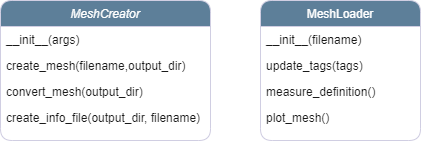
\includegraphics[width=0.5\textwidth]{Images/mesh_class.png}
    \caption{Classes and methods of \texttt{MeshUtils.py}.}
    \label{mesh_class}
\end{figure}

The \texttt{MeshCreator} constructor takes as input command-line arguments, for this reason the file contains also a \texttt{main} function where we use the \texttt{argparse} Python module to handle command-line arguments. 
The possible arguments that can be modified by the user are summarized in Table \ref{args}.

\begin{table}[H]
    \centering
    \begin{tabular}{|c|c|}
        \hline
        \textbf{Argument} & \textbf{Description} \\
        \hline
        nmesh & number of meshes to create \\
        nodes & number of nodes \\
        lc & characteristic length of the mesh \\
        hmax & maximum length of the interfaces \\
        hmin & minimum length of the interfaces \\
        seed & seed for random number generator \\
        spacing & boolean variable, True if the interfaces are equispaced \\
        wmax & maximum distance between the interfaces \\
        wmin & minimum distance between the interfaces \\
        \hline   
    \end{tabular}
    \caption{Command-line arguments.}
    \label{args}
\end{table}

The method \texttt{create\_mesh} generates nmesh new meshes using \texttt{gmsh} and the parameters passed to the constructor. The lengths of the intefaces are random numbers between hmin and hmax, while the distances between the interfaces are random numbers between wmin and wmax if the spacing argument is True, otherwhise they are equispaced and the distance is set equal to wmax. Different tags are assigned to the walls, the inlet boundary, the outlet boundary, each interface and each face. In the end, the meshes are saved in the \texttt{outpu\_dir} in \texttt{.msh} format.
At the end of this function, the \texttt{convert\_mesh} method is called to convert all the meshes in the \texttt{output\_dir} from \texttt{.msh} to \texttt{.xml} format. 

The last method of the class is \texttt{create\_info\_file} which is used to save a json file in the \texttt{output\_dir} containing the parameters used to generate the meshes.

The \texttt{MeshLoader} class is used to load a mesh from a \texttt{.xml} file. Teh constructor takes as input the name of the file and stores the following attributes:
\begin{itemize}
    \item \texttt{mesh}: FEniCS mesh object
    \item \texttt{bounds}: FEniCS \texttt{MeshFunction} associated to the boundaries of the mesh
    \item \texttt{face}: FEniCS \texttt{MeshFunction} associated to the faces of the mesh
    \item \texttt{n}: outward-pointing normal vector to the mesh boundaries
    \item \texttt{h}: minimun element size, used as characteristic length of the mesh
\end{itemize}

Another method of the class is \texttt{update\_tags(self,tags,nodes)}: this method can take as input a dictionary containing the tags of the mesh and the number of nodes of the graph (which is the number of interface plus the number of inlets and outlets). If the dictionary is not provided, the method computes automatically the tags dictionary based on the \texttt{nodes} input. The dictionary has the following structure: the keys are the strings 'walls', 'inlet', 'outlet', 'interface' and 'faces' and the values are lists containing the corresponding tags. 
If the number of nodes is not provided, the dictionary must be provided and it must have the same structure explained above.

Then the class has the \texttt{measure\_definition(self)} method: it return three \texttt{Mesure} FEniCS objects, which are used for integration over external boundaries, internal boundaries (interfaces) and faces. 

Finally, the mesh can be plotted using the \texttt{plot\_mesh(self)} method.

\subsection{Data generation}

\texttt{GenerateData.py} is located in the \texttt{scripts} folder and it contains two abstract classes: \texttt{Solver} and \texttt{DataGenerator}. The first one is used to solve the variational problem, while the second one is designed to store all the quantities of interest which will be used to build the graphs. Each of these parent classes has two child classes: we start describing the solver one.
A diagram of the \texttt{Solver} class structure and methods is shown in Figure \ref{solver_class}.

\begin{figure}[H]
    \centering
    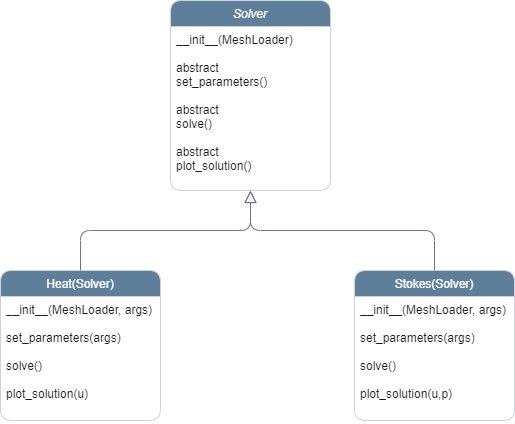
\includegraphics[width=0.5\textwidth]{Images/solver_class.png}
    \caption{\texttt{Solver} class structure and methods.}
    \label{solver_class}
\end{figure}

The abstract base class \texttt{Solver} contains the following methods:
\begin{itemize}
    \item \texttt{\(\twound\)init\(\twound\)(self,mesh)}: costructor that takes as input a \texttt{MeshLoader} object 
    \item \texttt{set\_parameters(self)}: abstract method
    \item \texttt{solve(self)}: abstract method
    \item \texttt{plot\_solution(self)}: abstract method
\end{itemize}

All the abstract method are overriden in the child classes \texttt{Heat} and \texttt{Stokes}. The choice of a parent abstract class for the solver is useful because it allows to use the same code for different problems, implementing child classes that solve different equations, but with the same structure. 
We focus on the description of the \texttt{Heat} class, since it is the one used in the test case, but the \texttt{Stokes} class is implemented analogously.

The \texttt{Heat} class contains the following methods overridden from the parent class:
\begin{itemize}
    \item \texttt{\(\twound\)init\(\twound\)(self,mesh, V, k, f, u0, dt, T, g, doplot=False)}: constructor which uses the \texttt{super()} function to inherit the base class constructor. The other problem parameters passed to the constructor are the function space, the diffusivity constant, the source term, the initial condition, the time step, the final step, the Neumann boundary condition at the inlet and a boolean variable to decide if the solution at each time step has to be plotted or not.
    \item \texttt{set\_parameters(self,V,k,f,u0,dt,T,g)}: function to set different problem parameters
    \item \texttt{solve(self)}: this method solves the Heat equation using Discontinuous Galerkin method, imposing a non-homogeneous Neumann condition at the inlet boundary and no-flux condition at the walls and at the outlet. The temperature at each time step is stored in a numpy array, as well as the time instants. 
    \item \texttt{plot\_solution(self,u)}: it takes as input the solution at a specific time step and it plots it.
\end{itemize}

\begin{figure}[H]
    \centering
    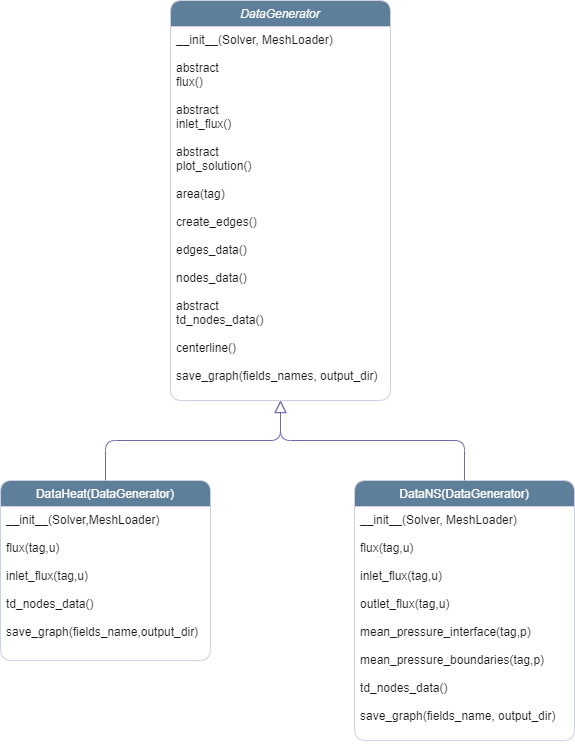
\includegraphics[width=0.5\textwidth]{Images/datagenerator_class.png}
    \caption{\texttt{DataGenerator} class structure and methods.}
    \label{datagenerator_class}
\end{figure}

The second abstract base class \texttt{DataGenerator} is schematized in Figure \ref{datagenerator_class}.

It contains the following methods:
\begin{itemize}
    \item \texttt{\(\twound\)init\(\twound\)(self,solver,mesh)}: constructor that takes as input a \texttt{Solver} object and a \texttt{MeshLoader} object. It saves \texttt{NNodes} as attribute of the object  which will be the number of nodes of the graph and it is set as the sum of the number of inlets, outlets and interfaces.
    \item \texttt{flux(self)}: abstract method 
    \item \texttt{inlet\_flux(self)}: abstract method
    \item \texttt{area(self,tag)}: concrete method that computes the area of the trapezoid corresponding to the tag passed as input 
    \item \texttt{nodes\_data(self)}: this function saves as attribute of the object a dictionary containing the time independent nodes features. The keys of the dictionary are strings with the name of the features and the values are numpy arrays containing the values at each node. The features considered for each node are the thermal diffusivity, the interface length where the node is located, the nodal type (inlet, outlet or branch node) and a global node ID.
    \item \texttt{td\_nodes\_data(self)}: abstract method
    \item \texttt{create\_edges(self)}: it stores as attributes of the object two numpy arrays (\texttt{self.edges1} and \texttt{self.edges2}) containing respectively the node IDs of the source nodes of every edge and the node IDs of the destination nodes.
    \item \texttt{edges\_data(self)}: it stores as attributes of the object a dictionary containing the edge feature. The dictionary structure is analogous to the one of the node features. The features saved are the distance between the nodes connected by the edge and the area of the trapezoid corresponding to the edge.
    \item \texttt{centerline(self)}: this function computes the coordinates of the graph nodes, which are the coordinates of the centerline of the mesh at the interfaces. These coordinates are stored in a numpy array of size \(NNodes \times 2\).
    \item \texttt{save\_graph(self, output\_dir,fields\_names)}: this method takes as input the name of the time dependent features of the graphs and the output directory where the graph has to be saves. It returns a dgl graph which is generated calling the functions defined in \texttt{generate\_graphs.py}, that will be described in the next section. 
    \item \texttt{generate\_json(output\_dir,model\_type)}: this function is used to generate and save in the output directory (that must be the directory containing the graphs) a json file containing information about the dataset. This file is necessary to make the dataset compatible with the gNN code. 
\end{itemize}

As for the \texttt{Solver} class, the abstract methods are overridden in the two child classes \texttt{DataNS}
and \texttt{DataHeat}. The \texttt{DataHeat} class includes these methods:
\begin{itemize}
    \item \texttt{\(\twound\)init\(\twound\)(self,solver,mesh)}: constructor inherited from the parent class. Two additional attributes are introduced: \texttt{model\_type} and \texttt{target\_fields}. The first one is a string containing the name of the equation considered, which is 'heat' in this case. The second one is a list containing the name of the time dependent features of the graph, which we call 'target features' since they are the features that the GNN has to predict. In this case the list contains only the string 'flux'.
    \item \texttt{flux(self,tag,u)}: method overridden from the parent class, it computes the heat flux of the solution \(u\) at the interface corresponding to the tag passed as input.
    \item \texttt{inlet\_flux(self,tag,u)}: method overridden from the parent class, it computes the heat flux at the inlet. The solution \(u\) and the tag of the inlet boundary are passe as input. 
    \item \texttt{td\_nodes\_data(self)}: methos overridden from the parent class, it stores as attribute of the object the time dependent nodes features in a dictionary. In this case the only time dependent feature is the heat flux: the dictionary has as key the time instant and as value a numpy array containing the heat flux at that time instant at each node.
    \item \texttt{save\_graphs(self, output\_dir)}: method that invokes the corresponding method of the parent class using the \texttt{super()} function, but the inputs \texttt{fields\_names} and \texttt{model\_type} are the \texttt{target\_fields} and \texttt{model\_type} attributes of the object.
    \item \texttt{generate\_json(self,output\_dir)}: method that invokes the corresponding method of the parent class using the \texttt{super()} function, but the \texttt{model\_type} input is the homonymous attribute of the object.
\end{itemize}

The \texttt{DataNS} is build analogously, with the only difference that the time dependent features are the flow rate and the pressure instead of the heat flux. In this case, the \texttt{flux} and \texttt{inlet\_flux} method computes the flow rate at the interfaces and at the inlet respectively. In addition, the class has a method \texttt{outlet\_flux} that computes the flow rate at the outlet and two other methods, \texttt{mean\_pressure\_interface} and \texttt{mean\_pressure\_boundaries}, that compute the mean pressure at the interfaces and at the inlet and outlet boundaries respectively.

\subsection{Graph generation}

In this section we describe the functions defined in \texttt{generate\_graphs.py}, included in the \texttt{scripts} folder, that are used to generate a dgl graph from the data obtained from the \texttt{DataGenerator} class. This file contains three functions: 
\begin{itemize}
    \item \texttt{generate\_graph(point\_data, points, edges\_data, edges1, edges2)}: this function takes as input a dictionary containing the time independent node features, a numpy array with the node coordinates, a dictionary containing the edge features and two numpy arrays containing the source and destination nodes of the edges. It return a dgl graph with the node and edge features stored as pytorch tensors.
    \item \texttt{add\_fields(graph, field, field\_name, offset=0)}: function to add a time dependent feature to the dgl graph. It take as input the dgl graph, a dictionary containing the field values at each time step, the name of the field to insert and an offset with the number of time steps to skip. It returns the dgl graph with the new field added.
    \item \texttt{save(filename, output\_dir)}: function to save the dgl graph in a file in the output directory.
\end{itemize}

All this function are invoked by the \texttt{save\_graph} method of the \texttt{DataGenerator} class, in this way a graph with all the necessary features is generated and saved in the output directory.

\subsection{Graph Neural Network}
\label{gnn}

In this section we describe the code of the graph neural network, located in the \texttt{gNN} folder. Since the code was already implemented and we just made some modifications, we will not describe it in detail, but we will focus on the changes we made and on the more relevant parts of the code, which are inside the \texttt{network1D} folder.

\subsubsection*{Code Structure}
To better understand the behavior of the network, it is necessary to look at its inner mechanisms. 
Starting from the \texttt{MLP} class, we can see that it is a simple multi-layer perceptron, with a number of hidden layers specified by the input parameter \texttt{n\_h\_layers}. This is the basic mechanism of all the network, every time that we want to process a node or an edge, we use an \texttt{MLP} to do so. 
The \texttt{MLP} class has a constructor that takes as input the number of input features, the number of output features, the size of the latent space and the number of hidden layers and use those inputs to create the input and output layers and the hidden layers. The input and output layers are \texttt{Linear} layers, while the hidden layers are \texttt{Linear} layers followed by a \texttt{LeakyReLU} activation function. 

The \texttt{MLP} class also has a \texttt{forward} method that computes the forward step of the network. It takes as input the input tensor and returns the result of the forward step. This is what will be meant when talking about encoding or decoding, feeding those data to an \texttt{MLP}.


The \texttt{EncodeProcessDecodeNetwork} class is the core of the network, it is the one that actually processes the graph. It is composed by three main parts: the encoder, the processor and the decoder. The encoder is composed by two \texttt{MLP}s, one for the nodes and one for the edges. The processor is made up by a number of \texttt{MLP}s equal to the number of iterations specified by the input parameter \texttt{process\_iterations}. The decoder is built using a single \texttt{MLP} that has the same number of neuron in its last layer as the output.

The \texttt{EncodeProcessDecodeNetwork} class constructor takes as input a dictionary of hyperparameters and uses it to initialize the encoder, the processor and the decoder. 
The \texttt{EncodeProcessDecodeNetwork} class also has five methods, one that encodes the edges (\texttt{encode\_edges}) and the other are for processing and decoding both edges and nodes (\texttt{process\_edges}, \texttt{process\_nodes}, \texttt{decode\_edges}, \texttt{decode\_nodes}). The attentive reader will surely notice that the method needed for encoding the nodes is missing, but this will become clear in the next paragraph.


The \texttt{MeshGraphNet} class is a subclass of \texttt{EncodeProcessDecodeNetwork}, it is the one that actually computes the pressure and flowrate updates given the previous system state. Its built using the same constructor as its father class. 

The method inside this class are the following:
\begin{itemize}
    \item \texttt{encode\_nodes}: this method takes as input the node features and returns the result of the encoding step. It is done inside this class to avoid losing generality in its parent class since nodes could have different features depending on the problem (e.g. \texttt{inlet\_mask} is quite specific to the fluid dynamics problem that this code originally solved).
    \item \texttt{continuity\_loss}: this method is not used in this test case, since we do not have any junction nodes. It is used to compute loss at junction nodes and it is left there to future proof the code.
    \item \texttt{forward}: this method is the one that actually computes the forward step of the network. It encodes both nodes and edges to the latent space, then perform a loop of processing iterations and finally decodes both nodes and edges to the output space. It returns the predicted update of the system state.
\end{itemize}

\subsubsection*{Training}

Here we describe the training process more in detail. The process is done using the \texttt{training.py} file and the \texttt{rollout.py} file. The first one is used to perform the steps necessary to train the network, like backpropagation and loss computation, while the second one is used to perform the forward step of the network and compute the predictions.

The training of the network starts with the definition of its hyperparameters described in Table \ref{hyperparams_description}. In particular, the first four parameters are the ones that define the network architecture, as explained in the previous section. The \texttt{rate\_noise} and \texttt{rate\_noise\_features} parameters are related to the noise that is added to the system state during the training process, to make the model more robust. The parameters listed in this table are the one from the original implementation, but we added some more to make the network more flexible, specifically a \texttt{n\_nout} parameter that defines the number of outputs of the network (and it must be equal to the number of target features) and a \texttt{bc\_type} which is a string that defines the type of boundary condition that has to be imposed (e.g. 'heat' in our test case).

\begin{table}[H]
\centering
\begin{tabular}{|l|l|}
\hline
\textbf{Parameter} & \textbf{Description} \\
\hline
latent\_size\_gnn & Size of the latent space of the Graph Neural Network \\
latent\_size\_mlp & Size of the latent space of each MLP \\
process\_iterations & Number of iterations of the process step \\
number\_hidden\_layers\_mlp & Number of hidden layers of each MLP \\
learning\_rate & Learning rate of the optimizer \\
batch\_size & Batch size \\
lr\_decay & Learning rate decay \\
nepochs & Number of epochs \\
weight\_decay & Weight decay for the optimizer \\
rate\_noise & Rate of noise \\
rate\_noise\_features & Rate of noise for the features \\
stride & Stride \\
\hline
\end{tabular}
\caption{Hyperparameters of the network.}
\label{hyperparams_description}
\end{table}

With all the hyperparameters set, we can start the training process. Since this part of the code was only modified by us, we will not go into much detail, but we will only describe the main steps. The training starts by taking a dataset composed of \texttt{DGL} graphs, which are split into a train set and a test set. Then are defined a loss (MSE) and a metric (MAE). The dataset is created in such a way that to train the network on all the graphs a map is needed so that when a single time-step is evaluated, the network is able to map that single time-step to the correct graph. The forward step is performed using the function \texttt{perform\_timestep} from the \texttt{rollout.py} file. This function takes as input the model, the graph and the previous time-step and predict the value of the quantity of interest at the next step in time. It also takes as input an array containing the boundary conditions and a boolean variable that indicates if the boundary conditions have to be imposed: if the boolean variable is True, the boundary conditions are imposed according to the \texttt{bc\_type} parameter.
This function is used also when evaluating the model since when we use it while training we compute the loss between the model's prediction and the ground truth, updating the weights of the network accordingly, while when we compute the rollout errors we use the model in inference mode and then compute the error between the prediction and the ground truth.

While the original implementation was meant to work only with blood flow data, we modified the original code so that, given a suitable dataset, it can be used to solve any problem. The main changes that we made are the following:
\begin{itemize}
    \item We modified the data generation part of the code to make it suitable for any kind of problem. In particular, we made sure that during the dataset creation, the \(N\) Quantities of Interest (QoI) are stored in the first \(N\) position of the dictionary containing the node features. This is done to make sure that the network can access the QoI easily. 
    \item We modified the dataset generation part in a way such that the program is able to create \(N\) deltas, one for each QoI. In this way we obtain our true update of the system state, which is the difference between the QoI at the current time-step and the QoI at the previous time-step. These deltas will be used to compute the loss of the network. 
    \item We modified the \texttt{training.py} file to make it able to take as input the number of outputs needed by the network. In this way we have completely generalized our library to be able to receive as input any suitable dataset.
\end{itemize}

With these modifications, the network is able to predict a variable number of QoI, which have to be specified by the user in the \texttt{main} function of the \texttt{training.py} file, in a list called \texttt{target\_features}. 
The limitation that persists despite of out changes, is the imposition of the boundary conditions. In fact, the network is able to impose only two types of boundary conditions that we called 'heat' and 'stokes', accordingly to the type of problems that we are solving in this work. Specifically, the 'heat' boundary condition that we used in the test case imposes the exact heat flux at the inlet node (Neumann boundary condition) and the zero heat flux at the outlet node (homogeneous Neumann boundary condition). If a new problem is considered, the user has to modify the \texttt{perform\_timestep} function in the \texttt{rollout.py} file in order to impose the correct boundary conditions.
    
\subsubsection*{Tester}
The \texttt{tester.py} file is used to test the trained model on graphs from the training and test set and on new graphs. The file is composed of the following already implemented functions: 
\begin{itemize}
    \item \texttt{get\_dataset\_and\_gnn}: loads the dataset and the trained GNN given a path to a saved model folder
    \item \texttt{get\_gnn\_and\_graphs}: loads the trained GNN and the graphs given a path to a saved model folder
    \item \texttt{evaluate\_all\_method}: computes the rollout phase for all the graphs in the dataset ('train' or 'test' is specified by the user), given a trained model. This function returns the average rollout error. 
\end{itemize}

In this file, we implemented two additional functions:
\begin{itemize}
    \item \texttt{plot\_predictions(dataset, split\_name, gnn\_model, params, graph\_idx=-1)}: it computes the rollout phase for a single graph and it plots the model's predictions compared to the real data, given a trained model and the dataset on which it was trained.
    It takes as input the dataset, the name of the split ('train' or 'test'), the trained model, the parameters of the model and the index of the graph to plot. If the index is not specified, the graph is randomly chosen. The function returns the nomalized error between the model's predictions and the real data.
    \item \texttt{evaluate\_new\_graph(path, graph\_name, graphs\_folder, data\_location)}: it computes the rollout phase and it plots the model's predictions and the real data for a new graph given a trained model. It takes as input the path to the model folder, the name of the graph to evaluate, the folder where the graph is stored and the path to the folder where the data are stored. As above, the function returns the average error of the rollout phase. Inside this method, the function \texttt{generate\_normalized\_graph} is called since we need to store the new graph features in order to evaluate the model.
\end{itemize}

\subsection{Notebooks}
To conclude the description of the code, we briefly explain the content of the notebooks in the \texttt{notebooks} folder. 

Firstly, there is the \texttt{HeatDatasetGen.ipynb} notebook, which is used to generate a dataset based on the Heat equation, as our test case. Inside this notebook, a random mesh is loaded from a given folder and the variational problem is solved using the \texttt{Heat} class, given a random diffusivity constant and the other parameters of the problem. Then, a graph is generated using the \texttt{DataHeat} class and it is saved in output directory. This process is repeated for a given number of times, in order to generate a dataset of graphs. Finally, the json file containing the information about the dataset is generated and saved in the same output directory. 

% Stokes notebook dobbiamo decidere se metterlo e cosa scriverci

Then, there is the \texttt{ModelTester.ipynb} which can be used to evaluate a trained model. In this notebook, it is necessary to specify the path to the model folder and the path to the proper dataset folder. In this way, the model and the dataser are both loaded and it is possible to visualize the predictions of the model on the graphs of the dataset and on new graphs from a different folder. It is also possible to display the average rollout errors on the train and test sets. All of this is done using the functions implemented in the \texttt{tester.py} file.

\section{Running instructions}

To run the code and reproduce the results presented in Section \ref{results}, it necessary to run the \texttt{ModelTester.ipynb} notebook. The path to our trained model and to the dataset that we used are already specified in the notebook, so it is not necessary to change them. It is possible to plot the predictions of the model on different graphs from the training and the test set just changing the index of the graph to plot. Then, the model's predictions on new graphs can be plotted just specifying the filename of a new graph and the folder where it is stored, some examples that can be tested are already specified in the notebook. 

Another possibility is to generate new meshes and new graphs, using the \texttt{MeshUtils.py} file and the \texttt{HeatDatasetGen.ipynb} notebook. 
First of all, new meshes can be created running the \texttt{main} function of the \texttt{MeshUtils.py} file from command-line. All the parameters that can be modified are listed in Table \ref{args} and they can be specified as command-line arguments. The directory where the meshes are saved and the mesh names can be modified in the \texttt{main} function. 
Then, the \texttt{HeatDatasetGen.ipynb} notebook can be used to generate a new dataset of graphs. It is necessary to specify the path to the folder containing the meshes, the path to the folder where the graphs have to be saved and the number of graphs to generate. Also, all the parameters of the variational problem can be modified in the notebook. 
Following these instructions, it is possible to evaluate the trained model on the new graphs generated using the \texttt{ModelTester.ipynb} notebook and specifying the name of the new graphs folder and the name of the graph to evaluate. Notice that it is necessary that the new graphs directory is inside the \texttt{data} folder.

For more details about the running instructions, to know about the packages required and for the training instructions, please refer to the README file in the repository.

%-----------------------------------------------------------------------------
% Results
%--- --------------------------------------------------------------------------

\section{Results}
\label{results}
In this section we show the results on the test case described in the section \ref{testcase}. 
In Figure \ref{loss} the performance of the model is shown in terms of loss and metric during the training. 
The loss function considered is the one defined in equation \ref{mse}, while the metric is the mean absolute error between the model's predictions and the real data. 
Moreover, the rollout error's behavior is shown in Figure \ref{rollout_plot} and it is computed as in Equation \ref{rollout} on a graph randomly selected in the dataset and at some random epochs. We can observe that the loss and the methic decreases during the training as expected, while the rollout error is not monotonically decreasing. This is due to the fact that the rollout error is computed on a single graph so it is not a good indicator of the model's performance.
In Table \ref{errors} we show the final rollout errors on the training and the test set, which are computed as the average of the rollout errorr on all the graphs in the dataset.

% immagini da aggiornare con quelle del modello finale
\begin{figure}[H]
    \centering
    \subfloat[Decay of loss function over 300 epochs.]{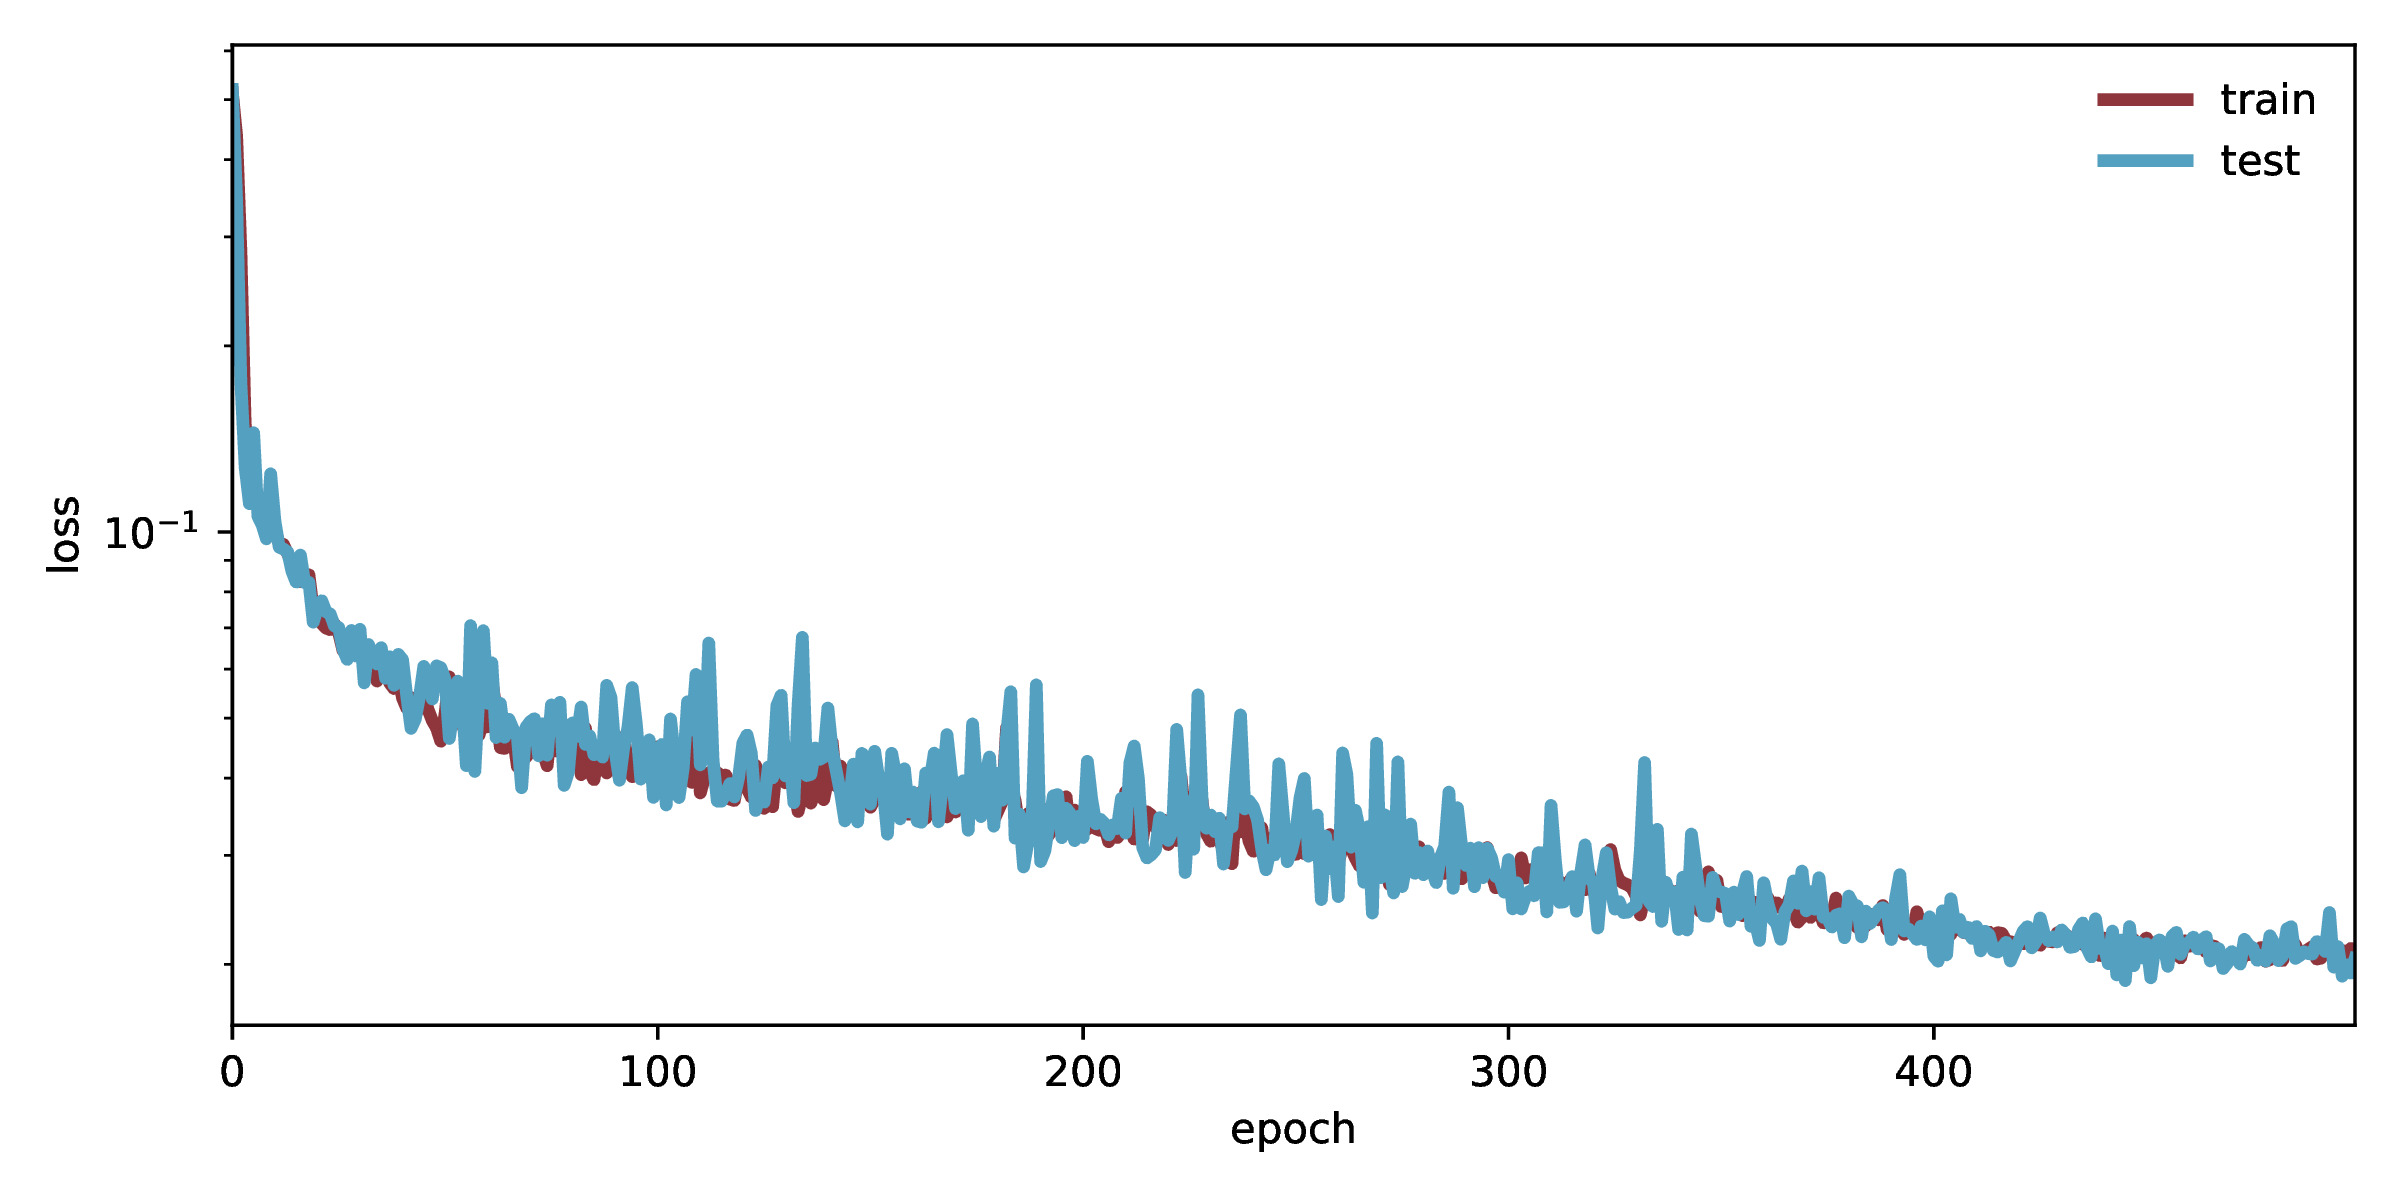
\includegraphics[width=0.45\textwidth]{Images/loss.jpg}}
    \subfloat[Decay of metric function over 300 epochs.]{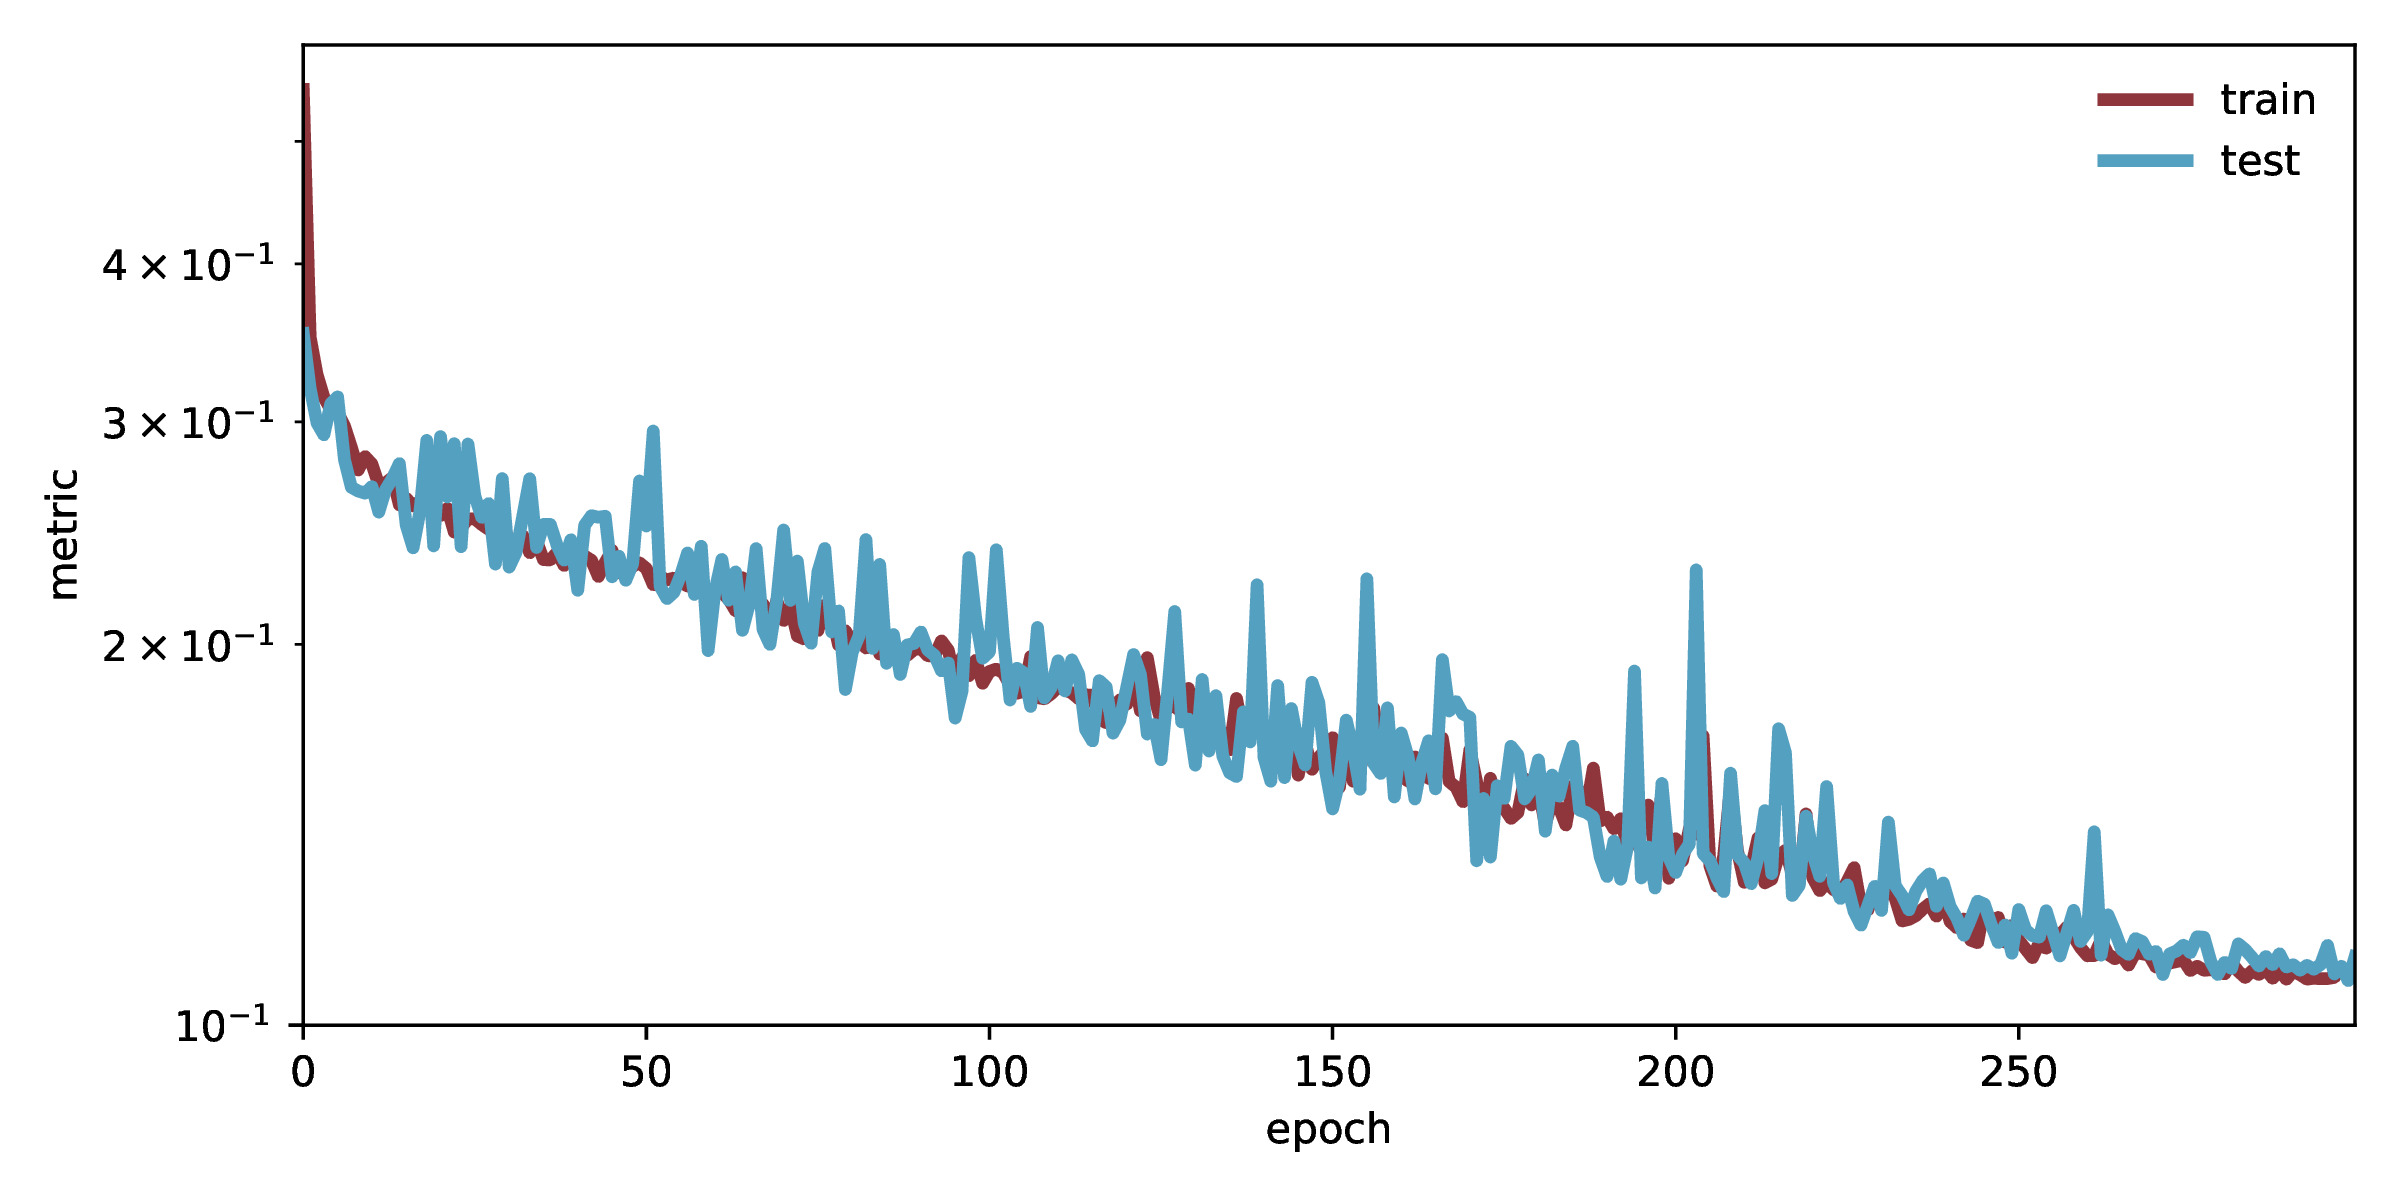
\includegraphics[width=0.45\textwidth]{Images/metric.jpg}}
    \caption{Loss and metric during the training.}
    \label{loss}
\end{figure}

\begin{figure}[H]
    \centering
    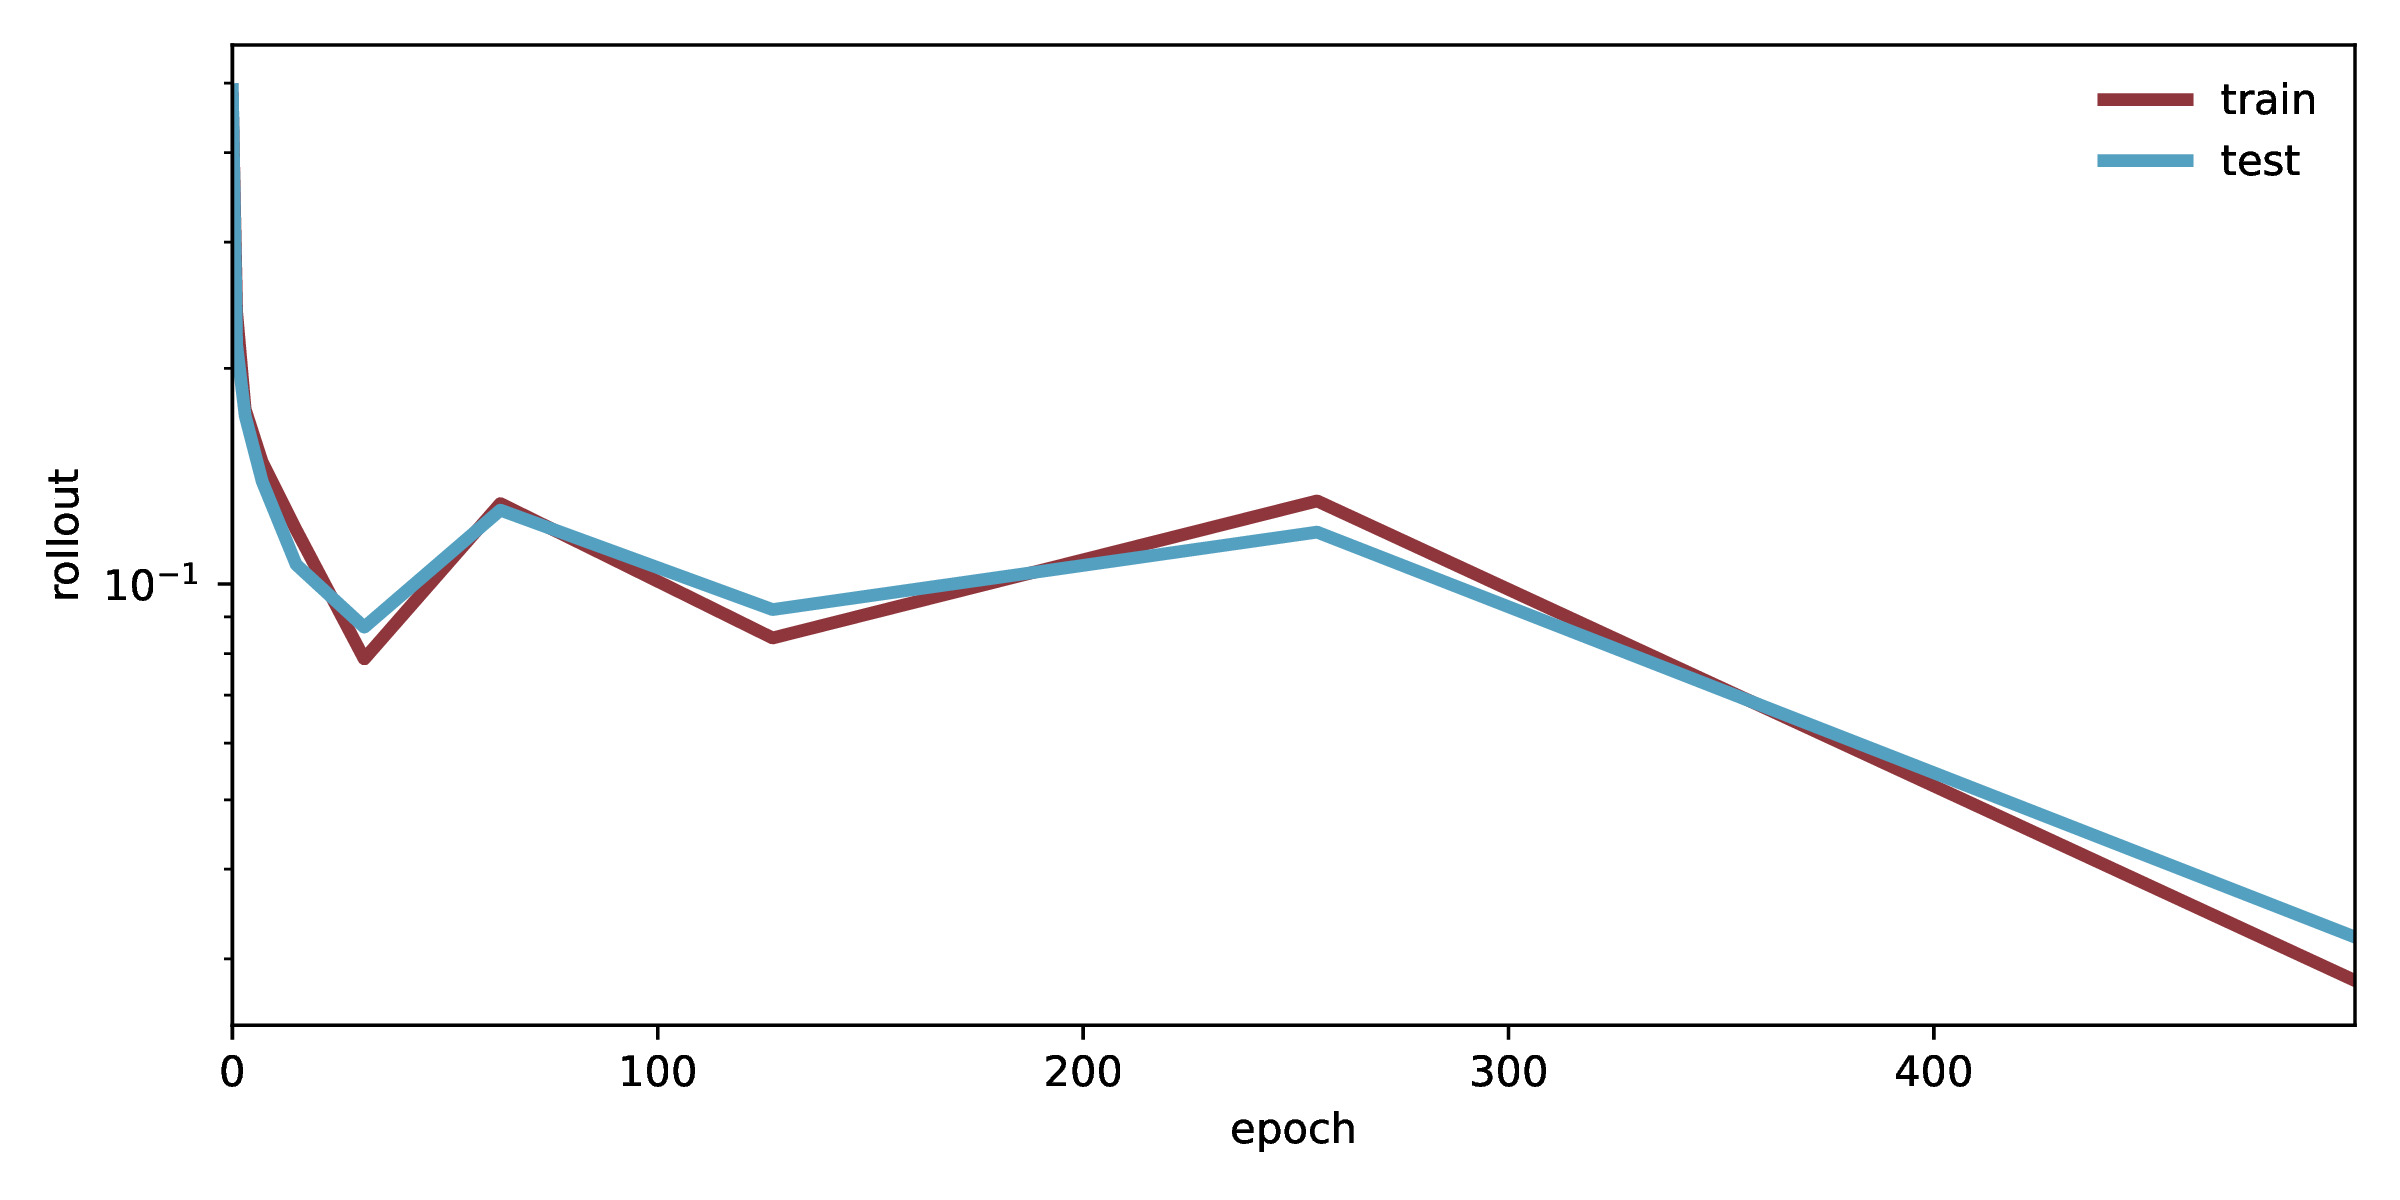
\includegraphics[width=0.6\textwidth]{Images/rollout.jpg}
    \caption{Rollout error over 300 epochs.}
    \label{rollout_plot}
\end{figure}

\begin{table}[H]
    \centering
    \begin{tabular}{|c|c|}
        \hline
        \textbf{Dataset} & \textbf{Rollout error} \\
        \hline
        Training & 0.031 \\
        Test & 0.033 \\
        \hline
    \end{tabular}
    \caption{Average rollout error on the training and the test set.}
    \label{errors}
\end{table}

In Figures \ref{train} and \ref{test} we can see some example of the model's predictions on each internal node of a graph from the training and the test set respectively. We don't show the predictions on the inlet and the outlet nodes since they are imposed by the boundary conditions and not predicted by the model.
In general, the model is able to predict the heat flux at the interfaces with good accuracy when we test it on graphs from the training and the test set. 

\begin{figure}[H]
    \centering
    \subfloat[Heat flux at interface 1.]{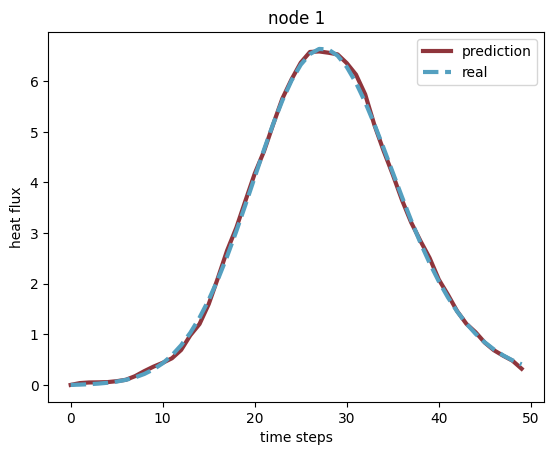
\includegraphics[width=0.3\textwidth]{Images/train_node1_k59.76.png}}
    \subfloat[Heat flux at interface 2.]{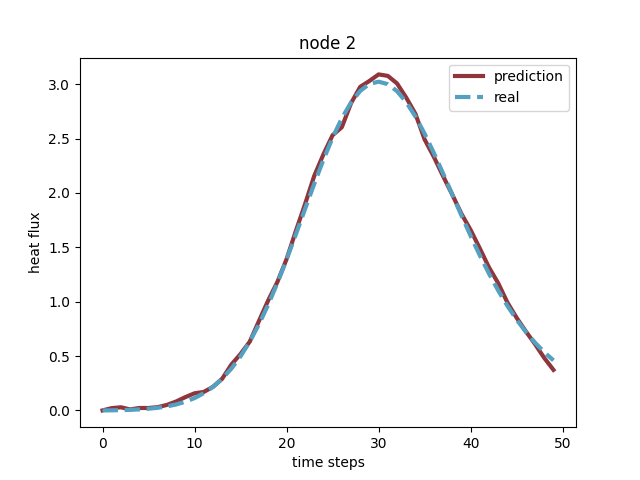
\includegraphics[width=0.3\textwidth]{Images/train_node2_k59.76.png}}
    \subfloat[Heat flux at interface 3.]{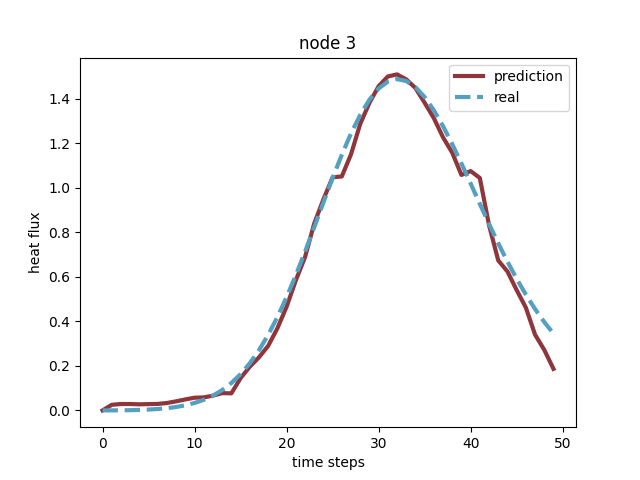
\includegraphics[width=0.3\textwidth]{Images/train_node3_k59.76.png}}
    \caption{Real heat flux at the interfaces predicted by the model on a graph from the training set with diffusivity constant \(k=59.76\).}
    \label{train}
\end{figure}

\begin{figure}[H]
    \centering
    \subfloat[Heat flux at interface 1.]{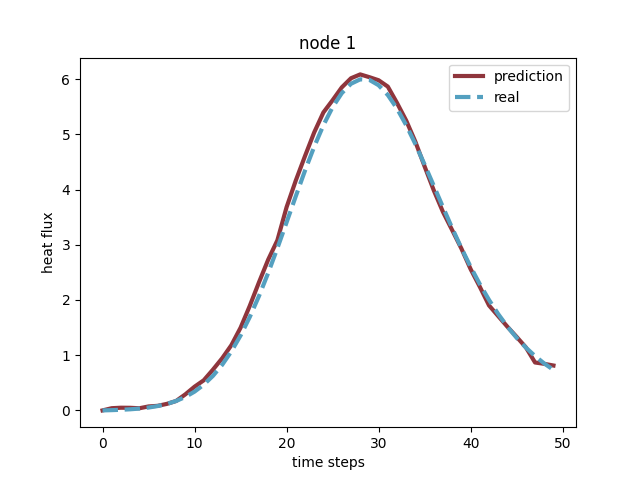
\includegraphics[width=0.3\textwidth]{Images/test_node1_k99.66.png}}
    \subfloat[Heat flux at interface 2.]{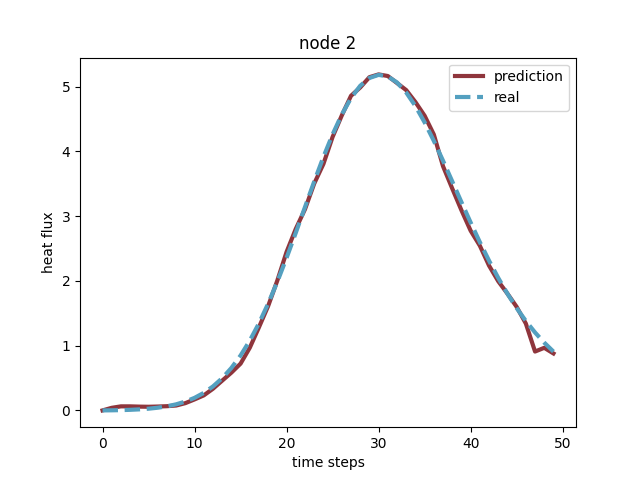
\includegraphics[width=0.3\textwidth]{Images/test_node2_k99.66.png}}
    \subfloat[Heat flux at interface 3.]{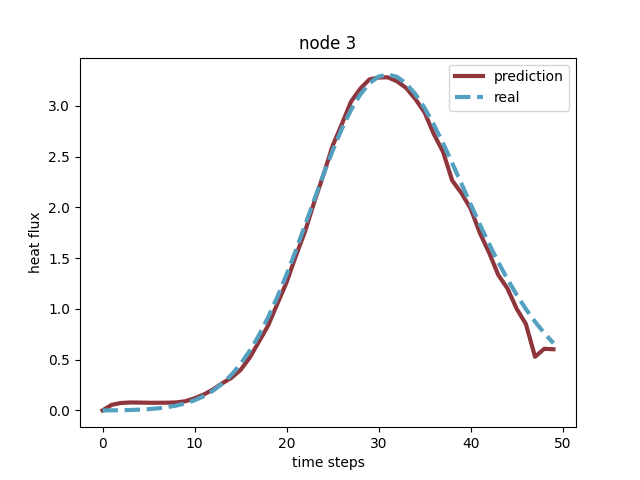
\includegraphics[width=0.3\textwidth]{Images/test_node3_k99.66.png}}
    \caption{Real heat flux at the interfaces predicted by the model on a graph from the test set with diffusivity constant \(k=99.66\).}
    \label{test}
\end{figure}

For a more accurate evaluation of the model's performance, we tested it on new graphs that were not included in the dataset. 
The predictions on these graphs compared to the real data are shown in Figures \ref{new1} and \ref{new2}. 
These graphs are generated solving the heat equations on different meshes and with different thermal conductivity constants with respect to the ones used to generate the dataset. 
We can observe that the predictions are more accurate on the nodes near to the inlet and less accurate on the nodes near to the outlet. 
Moreover, we have a slightly better performance on the graph with a higher \(k\). 
This could be due to the fact that with a lower diffusivity constant the values of the heat flux are smaller and the model has more difficulties in predicting them. The same argument can be applied to the nodes near to the outlet, where the heat flux is smaller with respect to the inlet.

\begin{figure}[H]
    \centering
    \subfloat[Heat flux at interface 1.]{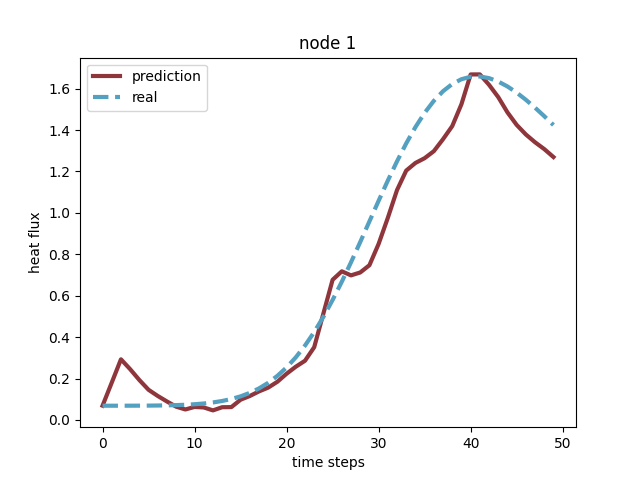
\includegraphics[width=0.3\textwidth]{Images/new_node1_k3.05.png}}
    \subfloat[Heat flux at interface 2.]{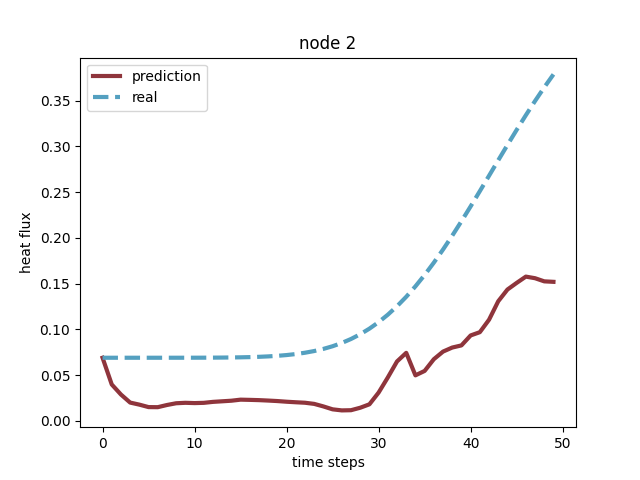
\includegraphics[width=0.3\textwidth]{Images/new_node2_k3.05.png}}
    \subfloat[Heat flux at interface 3.]{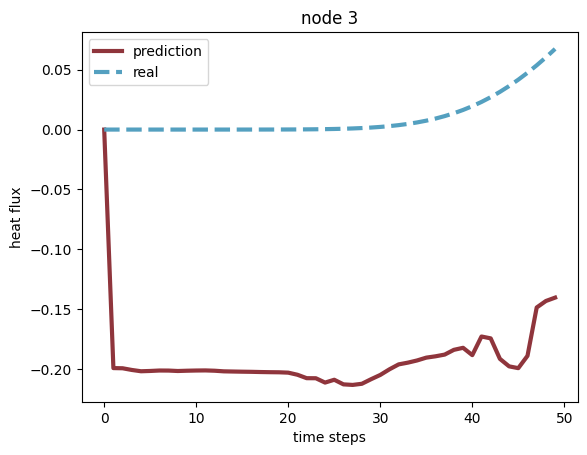
\includegraphics[width=0.3\textwidth]{Images/new_node3_k3.05.png}}
    \caption{Real heat flux at the interfaces predicted by the model on a new graph with diffusivity constant \(k=3.05\).}
    \label{new1}
\end{figure}

\begin{figure}[H]
    \centering
    \subfloat[subcaption]{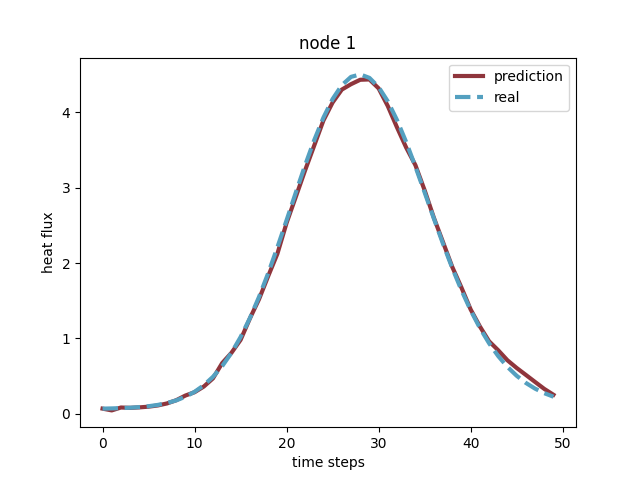
\includegraphics[width=0.3\textwidth]{Images/new_node1_k67.44.png}}
    \subfloat[subcaption]{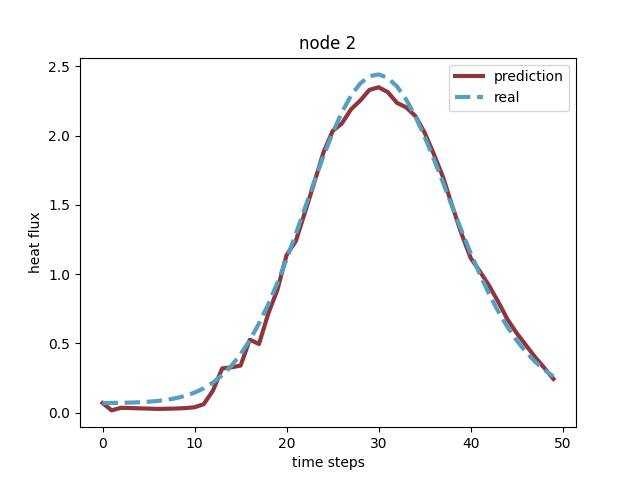
\includegraphics[width=0.3\textwidth]{Images/new_node2_k67.44.png}}
    \subfloat[subcaption]{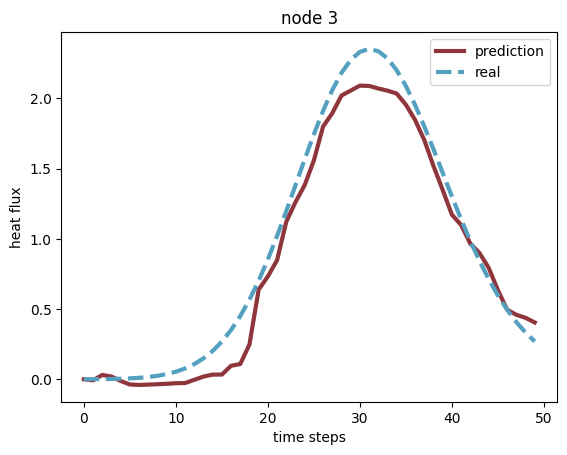
\includegraphics[width=0.3\textwidth]{Images/new_node3_k67.44.png}}
    \caption{Real heat flux at the interfaces predicted by the model on a new graph with diffusivity constant \(k=67.44\).}
    \label{new2}
\end{figure}

%-----------------------------------------------------------------------------
% Further work
%-----------------------------------------------------------------------------


\section{Further work and possible extensions}
In this work, we focused on a simple test case to show the potential of this approach, but it can be easily extended. We want to highlight that our model is not robust enough to be used in a real application, since it is trained on a very specific problem and on a dataset with a low variability. This could be improved in different ways.

First of all, in the dataset generation the variability of the datatset can be increased simply by changing the parameters of the mesh creation (for example considering not equally spaced interfaces or a higher number of interfaces) and also by changing other parameters of the problem in addition to the diffusivity constant (such as the inlet condition). 
In this way, the dataset will be more complex and the model will be more robust. 

In fact, our mesh creation code is limited to the generation of a specific type of mesh, with a single inlet and a single outlet. It could be interesting to extend it to generate more complex meshes, with more inlets and outlets, and also to generate meshes with bifucations and multiple branches, since the graph neural network code is already able to handle this kind of meshes. In this case, it would be necessary to modify the \texttt{DataGenerator} class to make it able to handle more complex meshes. 
Another easier modification can be to consider a 3-dimensional problem, instead of a 2-dimensional one, in order to make the model more realistic. Apart from the mesh creation, it would be necessary to modify only the \texttt{centerline}  function of the \texttt{DataGenerator}class to make it able to handle 3-dimensional meshes.

About the problems parameters of our test case, we considered only the diffusivity constant as a variable parameter, but it could be interesting to change also the other ones, such as the inlet condition or the source term, or even the time step and the final time. 

Another important extension is the possibility to consider different problems, such as the Stokes equation that we already implemented. We did not generate a dataset for this problem and we did not train the model on this problem for reasons of time, but it can be easily done. To do so, it woud be necessary to choose suitable problem parameters to generate a proper dataset. 
Once the dataset is generated, to train the graph neural network on the Stokes equation, it is necessary to modify the \texttt{main} function of the \texttt{training.py} file changing the target features to 'flowrate' and 'pressure', and also to modify the number of outputs of the network, which is a command-line argument. It is also required to modify the boundary conditions type in 'stokes', which is as well a command-line argument.

However, this is just an example to show how the code can be extended to other problems analogously, impleting a corresponding \texttt{Solver} class and a corresponding \texttt{DataGenerator} class, inherited from the parent classes, and modifying the \texttt{main} function of the \texttt{training.py} file with the proper target, nodes and edges features. In this case, it may be necessary to change how the boundary conditions are imposed accordingly to the problem considered (it can be done in the \texttt{perform\_timestep} function of the \texttt{rollout.py} file). This is the main limitation in the gNN code that has to be fixed manually by the user when a new problem is considered. 

To conclude, in this work we have managed to implement a fully working pipeline from mesh and dataset generation to training and testing of a graph neural network. In this way, we have shown that this approach can be used to solve a wide range of problems, from fluid dynamics to heat transfer. We believe that this could be a very powerful tool for simulations of complex problems, where the use of traditional numerical methods and of 3-dimensional models is not feasible.


%---------------------------------------------------------------------------
%  BIBLIOGRAPHY
%---------------------------------------------------------------------------
\newpage
% Remember to insert here only the essential bibliography of your work
\bibliography{bibliography.bib} % automatically inserted and ordered with this command

\end{document}
